\documentclass[journal,10pt,twocolumn]{article}
\usepackage{graphicx}
\usepackage[margin=0.8in]{geometry}
\usepackage[cmex10]{amsmath}
\usepackage{array}
\usepackage{booktabs}
\usepackage{mathtools}
\title{\textbf{Construction assignment}}
\author{Mohamed Hamdan}
\date{September 2022}


\providecommand{\norm}[1]{\left\lVert#1\right\rVert}
\providecommand{\abs}[1]{\left\vert#1\right\vert}
\let\vec\mathbf
\newcommand{\myvec}[1]{\ensuremath{\begin{pmatrix}#1\end{pmatrix}}}
\newcommand{\mydet}[1]{\ensuremath{\begin{vmatrix}#1\end{vmatrix}}}
\providecommand{\brak}[1]{\ensuremath{\left(#1\right)}}
\providecommand{\lbrak}[1]{\ensuremath{\left(#1\right.}}
\providecommand{\rbrak}[1]{\ensuremath{\left.#1\right)}}
\providecommand{\sbrak}[1]{\ensuremath{{}\left[#1\right]}}

\begin{document}

\maketitle
\paragraph{\textit{Problem Statement} - Construct a quadilateral circumscribing a circle}

\section*{\large Solution}

\begin{figure}[h]
\centering
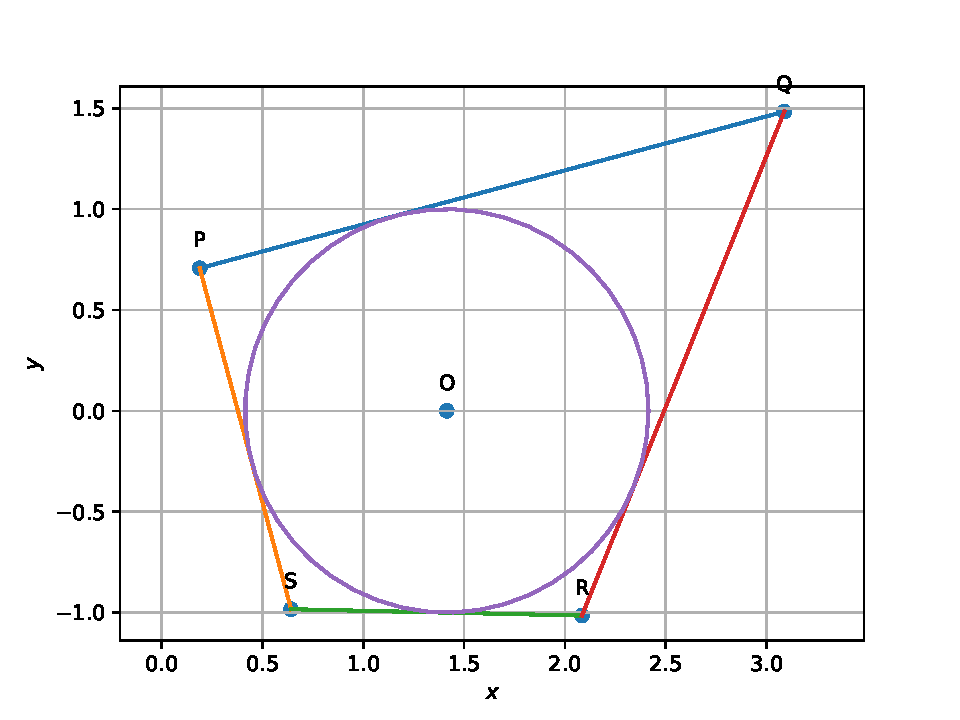
\includegraphics[width=1\columnwidth]{figs/fig1.pdf}
\caption{Quadilateral circumscribing a circle}
\label{fig:circ_quad}
\end{figure}

Select a point $\vec{P}$ from which two tangents are drawn to the circle with center $\vec{O}$ and radius $r$. The direction vectors $\vec{m_i}$ satisfy the equation
\begin{align}
	\vec{m}_i^\top\vec{\Sigma}\vec{m}_i = 0
\end{align}
Assuming the external point as $\vec{h}$, $\vec{\Sigma}$ is given by
\begin{align}
	\label{eq:Sigma}
	\vec{\Sigma} = \brak{\vec{Vh}+\vec{u}}\brak{\vec{Vh}+\vec{u}}^\top - \brak{\vec{h}^\top\vec{V}\vec{h} + 2\vec{u}^\top\vec{h} + f}\vec{V}
\end{align}
$\vec{\Sigma}$ can be orthogonally diagonalized as
\begin{align}
	\label{eq:Sigma_diag}
	\vec{\Sigma} &= \vec{\Gamma}^\top\vec{D}\vec{\Gamma}\\
	\label{eq:eigevalV}
	\vec{D} &= \myvec{\lambda_1 & 0\\ 0 & \lambda_2}, \\
	\label{eq:eigevecP}
	\vec{\Gamma} &= \myvec{\vec{y}_1 & \vec{y}_2}, \quad \vec{\Gamma}^{\top}=\vec{\Gamma}^{-1}
\end{align}
Using \eqref{eq:eigevalV} and \eqref{eq:eigevecP} and substituting $\vec{h}$ as $\vec{P}$, the normal vectors $\vec{n}_i$ of the tangents drawn from $\vec{P}$ can be written as
\begin{align}
	\label{eq:tangent_normals}
	\vec{n}_i = \vec{\Gamma}\myvec{\sqrt{\abs{\lambda_1}} \\\\ \pm\sqrt{\abs{\lambda_2}}}
\end{align}
Using the vectors $\vec{n}_i$ in \eqref{eq:tangent_normals}, the direction vectors $\vec{m}_i$ can be found in 2-dimensional space since they are orthogonal. The points of contact of the tangents are then given by
\begin{align}
	\vec{T}_i = \vec{P} - \frac{\vec{m}_i^\top\brak{\vec{VP}+\vec{u}}}{\vec{m}_i^\top\vec{V}\vec{m}_i}
\end{align}
Where $\vec{T}_i$ are the points of contact. Consider two direction vectors $\vec{t}_1$ and $\vec{t}_2$ as
\begin{align}
	\vec{t}_1 &= \vec{T}_1 - \vec{P}\\
	\vec{t}_2 &= \vec{T}_2 - \vec{P}
\end{align}
The points $\vec{Q}$ and $\vec{S}$ can then be found as
\begin{align}
	\label{eq:pt_Q}
	\vec{Q} &= \vec{P} + \mu_1\vec{t}_1\\ 
	\label{eq:pt_S}
	\vec{S} &= \vec{P} + \mu_2\vec{t}_2
\end{align}
Where $\mu_i$ are the parameters for the distance of points $\vec{Q}$ and $\vec{S}$ from point $\vec{P}$.\\\\
Each of the vectors $\vec{n}_i$ are also normal vectors to one of the tangents from $\vec{Q}$ and $\vec{S}$ from \eqref{eq:pt_Q} and \eqref{eq:pt_S}. By using \eqref{eq:Sigma_diag} and \eqref{eq:tangent_normals}, the normal vectors for tangents from $\vec{Q}$ and $\vec{S}$ and not passing through $\vec{P}$ can be found by using the 
condition
\begin{align}
	\label{eq:diff_normal_cond}
	\norm{\vec{k}_i\times\vec{n}_i} \neq 0   
\end{align}
where $\vec{k}_i$ are the normal vectors of interest.
The point $\vec{R}$ can then be found as the intersection of lines given by
\begin{align}
	\label{eq:distinct_tangent_Q}
	\vec{k}_1^\top\brak{\vec{x}-\vec{Q}} &= 0\\
	\label{eq:distinct_tangent_S}
	\vec{k}_2^\top\brak{\vec{x}-\vec{S}} &= 0
\end{align}
Solving \eqref{eq:distinct_tangent_Q} and \eqref{eq:distinct_tangent_S} with $\vec{x}$ as point $\vec{R}$, we get
\begin{align}
	\label{eq:point_R_soln}
	\vec{R} = \myvec{\vec{k}_1^\top \\\\ \vec{k}_2^\top}^{-1}\myvec{\vec{k}_1^\top\vec{Q} \\\\ \vec{k}_2^\top\vec{S}}
\end{align}
\end{document}
